\documentclass[en]{university}

\usepackage {tikz}
\usetikzlibrary {positioning}
\definecolor {processblue}{cmyk}{0.96,0,0,0}

\faculty{Department of Computer Engineering}
\course{Computer Networks}
\subject{Homework 3}
\professor{Dr. Jafari}
\student{Parsa Mohammadian}

\begin{document}

\setupdocument

\section{}
Software-Defined Networking or SDN is a networking architecture that uses software-based controllers or APIs\footnote{Application Programming Interface} to implement network functions for hardware-based infrastructure.

The architecture of SDN is shown in Figure \ref{fig:sdn}. Since the control layer of network is decoupled from the infrastructure layer, SDN has the following criterias:
\begin{itemize}
    \item Directly programmable
    \item Agile
    \item Centerally managed
    \item Programmatically configured
    \item Open standard-based and vendor neutral
\end{itemize}
SDN can be implementd in three main ways:
\begin{itemize}
    \item Open SDN: The controller comunicates with the switches using OpenFlow protocol as shown in Figure \ref{fig:open-sdn}.
    \item SDN via APIs: The functions in remote devices are implemented using APIs(SNMP, CLI, Rest, \dots) as shown in Figure \ref{fig:sdn-api}.
    \item SDN via hypervisor-based overlay network: Hypervisor-based overlay networks are created over the top of the physical network. The hypervisor is responsible for the control layer of the network as shown in Figure \ref{fig:sdn-hyper}.
\end{itemize}
\begin{figure}
    \centering
    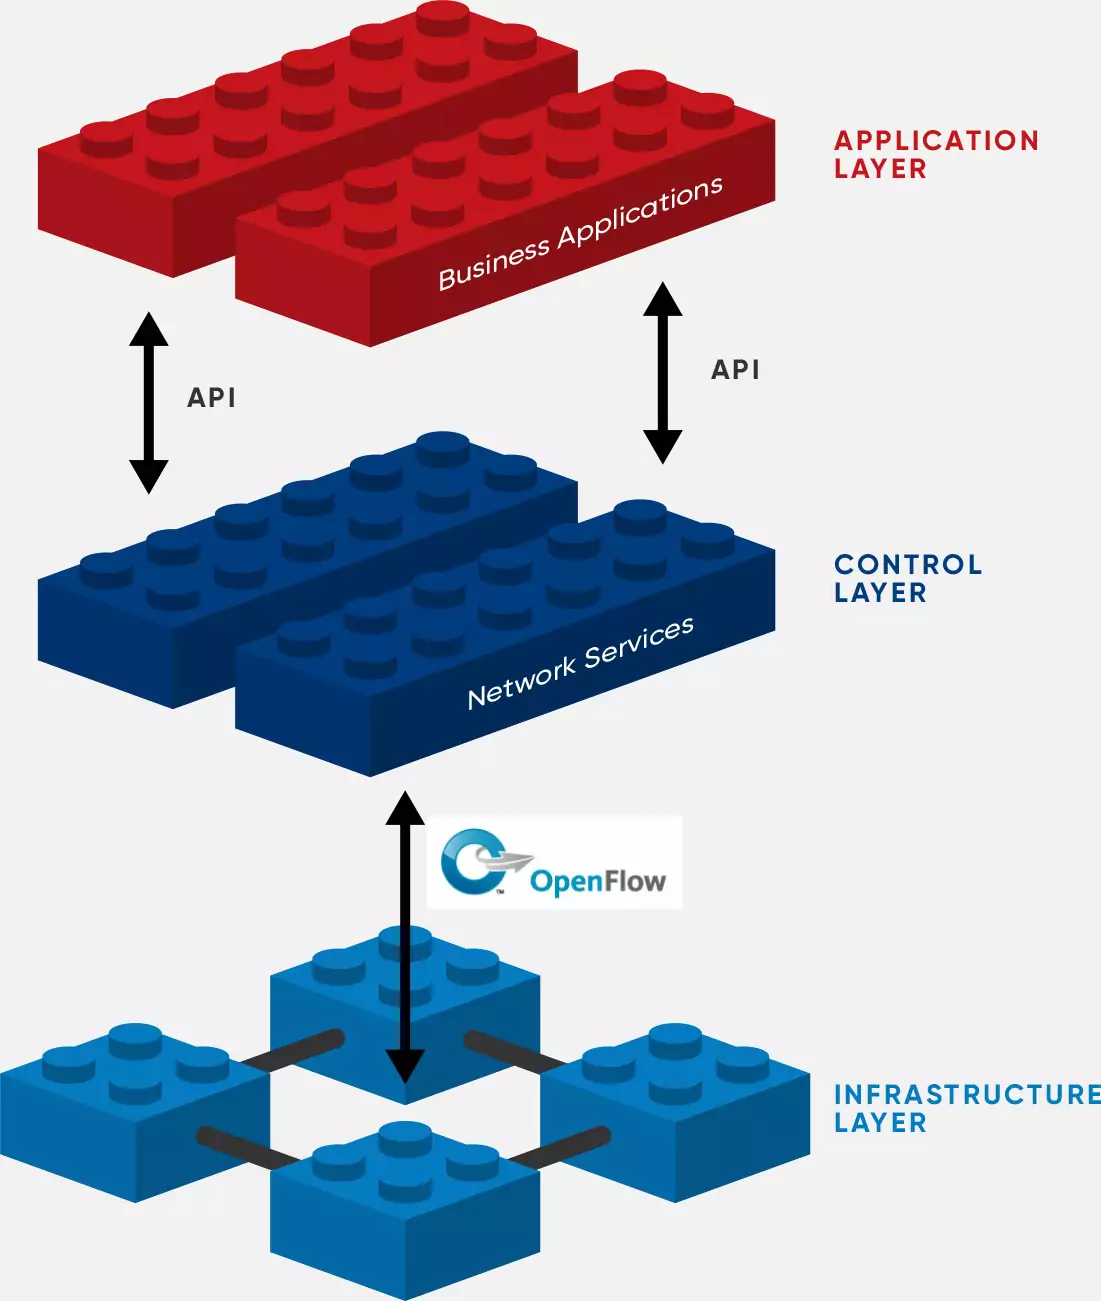
\includegraphics[width=0.8\textwidth]{resources/sdn-architecture-img.png}
    \caption{SDN Architecture}
    \label{fig:sdn}
\end{figure}
\begin{figure}
    \centering
    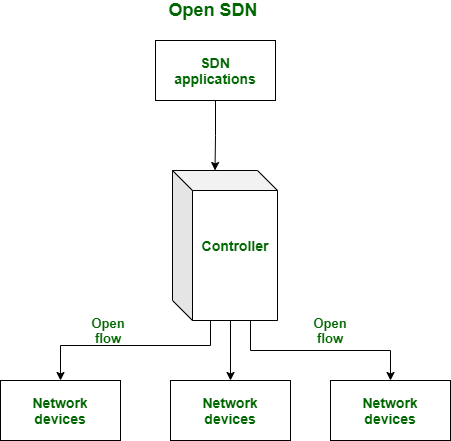
\includegraphics[width=0.8\textwidth]{resources/OpenSDNdrawio.png}
    \caption{Open SDN}
    \label{fig:open-sdn}
\end{figure}
\begin{figure}
    \centering
    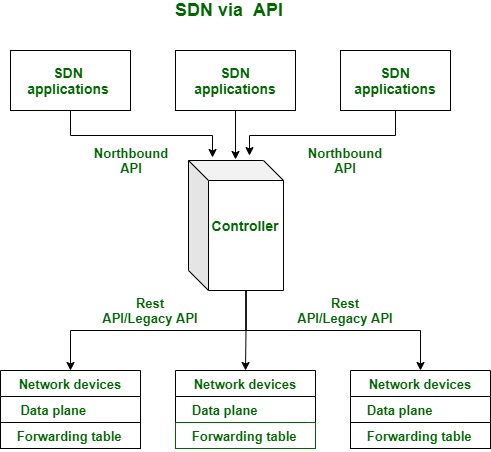
\includegraphics[width=0.8\textwidth]{resources/SDNAPIdrawio.png}
    \caption{SDN via APIs}
    \label{fig:sdn-api}
\end{figure}
\begin{figure}
    \centering
    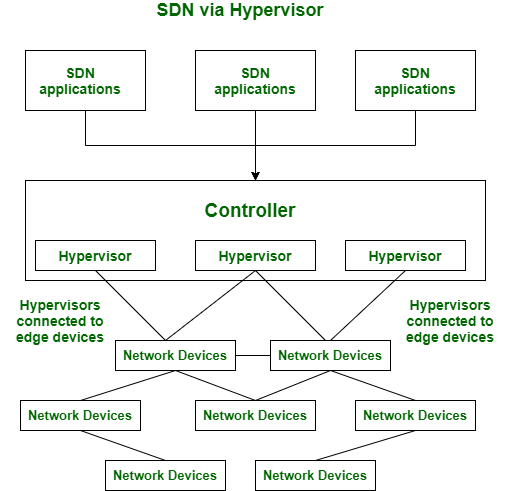
\includegraphics[width=0.8\textwidth]{resources/SDNviahypervisordrawio.png}
    \caption{SDN via hypervisor-based overlay network}
    \label{fig:sdn-hyper}
\end{figure}
SDN advantages:
\begin{itemize}
    \item Centeralized controller
    \item Reduced lines of configuration code due to seperation of data and control plane
    \item The code is written only once and can be used in multiple environments
    \item The controller features can eliminate the need for external devices and overaly reduce the cost of the network
    \item Openness
\end{itemize}

\subsubsection*{Resources}
\begin{itemize}
    \item \href{https://youtube.com/watch?v=Z5Gi2Bpd82M}{\url{https://youtube.com/watch?v=Z5Gi2Bpd82M}}
    \item \href{https://youtube.com/watch?v=Nh2hXUuKXyQ}{\url{https://youtube.com/watch?v=Nh2hXUuKXyQ}}
    \item \href{https://opennetworking.org/sdn-definition/}{\url{https://opennetworking.org/sdn-definition/}}
    \item \href{https://www.geeksforgeeks.org/types-of-software-defined-networks-implementation/}{\url{https://www.geeksforgeeks.org/types-of-software-defined-networks-implementation/}}
\end{itemize}

\section{}
\subsection{}
Telegram normal messages use server-client/client-server encryption. It means they are secure while transmitting between clients and servers in a way that only the server and the client can decrypt the message.
Then in the server all this messages are stored in a secure database. This way Telegram allows multiple clients to connect as a same user.
On the other hand, Telegram secret chats are client-client encrypted. At the start of the secret chat, participants exchange encryption keys.
Then the messages are encrypted using the keys exchanged.
This means that only two sides of the conversation can decrypt the message. In such a case, the server can not decrypt the message at all. Because of that, newly connected clients can not access the secret chat.
\subsubsection*{Resources}
\begin{itemize}
    \item \href{https://telegram.org/faq}{\url{https://telegram.org/faq}}
\end{itemize}

\subsection{}
As mentioned in official WhatsApp documentation, WhatsApp uses end-to-end encryption. This is just like Telegram secret chats.
Actually, this is the main reason why WhatsApp can not restore your messages on newly connected clinet if you lost all your logged in devices.
So WhatsApp is not peer-to-peer.
\subsubsection*{Resources}
\begin{itemize}
    \item \href{https://www.whatsapp.com/security/}{\url{https://www.whatsapp.com/security/}}
\end{itemize}

\section{}
\subsection{}
\begin{table}[H]
    \centering
    \caption{Link State Routing}
    \label{tab:dijkstra}
    \begin{tabular}{|*6{c|}}
        \hline
        Step & $N'$                  & $D(R_2),P(R_2)$ & $D(R_3),P(R_3)$ & $D(R_4),P(R_4)$ & $D(R_5),P(R_5)$ \\
        \hline
        1    & $R_1$                 & $5,R_1$         & $\infty$        & $2,R_1$         & $\infty$        \\
        2    & $R_1 R_4$             & $3,R_4$         & $3,R_4$         &                 & $5,R_4$         \\
        3    & $R_1 R_4 R_2$         &                 & $3,R_4$         &                 & $5,R_4$         \\
        4    & $R_1 R_4 R_2 R_3$     &                 &                 &                 & $5,R_4$         \\
        5    & $R_1 R_4 R_2 R_3 R_5$ &                 &                 &                 &                 \\
        \hline
    \end{tabular}
\end{table}

\subsection{}
\begin{minipage}[t]{0.5\textwidth}
    \begin{table}[H]
        \centering
        \caption{Distance Vector Step 1}
        \label{tab:dvr1}
        \begin{tabular}{c|*5c}
            $R_1$ Table & $R_1$    & $R_2$    & $R_3$    & $R_4$    & $R_5$    \\
            \hline
            $R_1$       & $0$      & $5$      & $\infty$ & $2$      & $\infty$ \\
            $R_2$       & $\infty$ & $\infty$ & $\infty$ & $\infty$ & $\infty$ \\
            $R_3$       & $\infty$ & $\infty$ & $\infty$ & $\infty$ & $\infty$ \\
            $R_4$       & $\infty$ & $\infty$ & $\infty$ & $\infty$ & $\infty$ \\
            $R_5$       & $\infty$ & $\infty$ & $\infty$ & $\infty$ & $\infty$
        \end{tabular}
        \begin{tabular}{c|*5c}
            $R_2$ Table & $R_1$    & $R_2$    & $R_3$    & $R_4$    & $R_5$    \\
            \hline
            $R_1$       & $\infty$ & $\infty$ & $\infty$ & $\infty$ & $\infty$ \\
            $R_2$       & $5$      & $0$      & $4$      & $1$      & $\infty$ \\
            $R_3$       & $\infty$ & $\infty$ & $\infty$ & $\infty$ & $\infty$ \\
            $R_4$       & $\infty$ & $\infty$ & $\infty$ & $\infty$ & $\infty$ \\
            $R_5$       & $\infty$ & $\infty$ & $\infty$ & $\infty$ & $\infty$
        \end{tabular}
        \begin{tabular}{c|*5c}
            $R_3$ Table & $R_1$    & $R_2$    & $R_3$    & $R_4$    & $R_5$    \\
            \hline
            $R_1$       & $\infty$ & $\infty$ & $\infty$ & $\infty$ & $\infty$ \\
            $R_2$       & $\infty$ & $\infty$ & $\infty$ & $\infty$ & $\infty$ \\
            $R_3$       & $\infty$ & $4$      & $0$      & $1$      & $2$      \\
            $R_4$       & $\infty$ & $\infty$ & $\infty$ & $\infty$ & $\infty$ \\
            $R_5$       & $\infty$ & $\infty$ & $\infty$ & $\infty$ & $\infty$
        \end{tabular}
        \begin{tabular}{c|*5c}
            $R_4$ Table & $R_1$    & $R_2$    & $R_3$    & $R_4$    & $R_5$    \\
            \hline
            $R_1$       & $\infty$ & $\infty$ & $\infty$ & $\infty$ & $\infty$ \\
            $R_2$       & $\infty$ & $\infty$ & $\infty$ & $\infty$ & $\infty$ \\
            $R_3$       & $\infty$ & $\infty$ & $\infty$ & $\infty$ & $\infty$ \\
            $R_4$       & $2$      & $1$      & $1$      & $0$      & $3$      \\
            $R_5$       & $\infty$ & $\infty$ & $\infty$ & $\infty$ & $\infty$
        \end{tabular}
        \begin{tabular}{c|*5c}
            $R_5$ Table & $R_1$    & $R_2$    & $R_3$    & $R_4$    & $R_5$    \\
            \hline
            $R_1$       & $\infty$ & $\infty$ & $\infty$ & $\infty$ & $\infty$ \\
            $R_2$       & $\infty$ & $\infty$ & $\infty$ & $\infty$ & $\infty$ \\
            $R_3$       & $\infty$ & $\infty$ & $\infty$ & $\infty$ & $\infty$ \\
            $R_4$       & $\infty$ & $\infty$ & $\infty$ & $\infty$ & $\infty$ \\
            $R_5$       & $\infty$ & $\infty$ & $2$      & $3$      & $0$
        \end{tabular}
    \end{table}
\end{minipage}
\begin{minipage}[t]{0.5\textwidth}
    \begin{table}[H]
        \centering
        \caption{Distance Vector Step 2}
        \label{tab:dvr2}
        \begin{tabular}{c|*5c}
            $R_1$ Table & $R_1$    & $R_2$    & $R_3$    & $R_4$    & $R_5$    \\
            \hline
            $R_1$       & $0$      & $3$      & $3$      & $2$      & $5$      \\
            $R_2$       & $5$      & $0$      & $4$      & $1$      & $\infty$ \\
            $R_3$       & $\infty$ & $\infty$ & $\infty$ & $\infty$ & $\infty$ \\
            $R_4$       & $2$      & $1$      & $1$      & $0$      & $3$      \\
            $R_5$       & $\infty$ & $\infty$ & $\infty$ & $\infty$ & $\infty$
        \end{tabular}
        \begin{tabular}{c|*5c}
            $R_2$ Table & $R_1$    & $R_2$    & $R_3$    & $R_4$    & $R_5$    \\
            \hline
            $R_1$       & $0$      & $5$      & $\infty$ & $2$      & $\infty$ \\
            $R_2$       & $3$      & $0$      & $2$      & $1$      & $4$      \\
            $R_3$       & $\infty$ & $4$      & $0$      & $1$      & $2$      \\
            $R_4$       & $2$      & $1$      & $1$      & $0$      & $3$      \\
            $R_5$       & $\infty$ & $\infty$ & $\infty$ & $\infty$ & $\infty$
        \end{tabular}
        \begin{tabular}{c|*5c}
            $R_3$ Table & $R_1$    & $R_2$    & $R_3$    & $R_4$    & $R_5$    \\
            \hline
            $R_1$       & $\infty$ & $\infty$ & $\infty$ & $\infty$ & $\infty$ \\
            $R_2$       & $5$      & $0$      & $4$      & $1$      & $\infty$ \\
            $R_3$       & $3$      & $2$      & $0$      & $1$      & $2$      \\
            $R_4$       & $2$      & $1$      & $1$      & $0$      & $3$      \\
            $R_5$       & $\infty$ & $\infty$ & $2$      & $3$      & $0$
        \end{tabular}
        \begin{tabular}{c|*5c}
            $R_4$ Table & $R_1$    & $R_2$    & $R_3$    & $R_4$ & $R_5$    \\
            \hline
            $R_1$       & $0$      & $5$      & $\infty$ & $2$   & $\infty$ \\
            $R_2$       & $5$      & $0$      & $4$      & $1$   & $\infty$ \\
            $R_3$       & $\infty$ & $4$      & $0$      & $1$   & $2$      \\
            $R_4$       & $2$      & $1$      & $1$      & $0$   & $3$      \\
            $R_5$       & $\infty$ & $\infty$ & $2$      & $3$   & $0$
        \end{tabular}
        \begin{tabular}{c|*5c}
            $R_5$ Table & $R_1$    & $R_2$    & $R_3$    & $R_4$    & $R_5$    \\
            \hline
            $R_1$       & $\infty$ & $\infty$ & $\infty$ & $\infty$ & $\infty$ \\
            $R_2$       & $\infty$ & $\infty$ & $\infty$ & $\infty$ & $\infty$ \\
            $R_3$       & $\infty$ & $4$      & $0$      & $1$      & $2$      \\
            $R_4$       & $2$      & $1$      & $1$      & $0$      & $3$      \\
            $R_5$       & $5$      & $4$      & $2$      & $3$      & $0$
        \end{tabular}
    \end{table}
\end{minipage}
\begin{table}[H]
    \centering
    \caption{Distance Vector Step 3 (Final)}
    \label{tab:dvr3}
    \begin{tabular}{c|*5c}
        $R_1$ Table & $R_1$ & $R_2$ & $R_3$ & $R_4$ & $R_5$ \\
        \hline
        $R_1$       & $0$   & $3$   & $3$   & $2$   & $5$   \\
        $R_2$       & $3$   & $0$   & $2$   & $1$   & $4$   \\
        $R_3$       & $3$   & $4$   & $0$   & $1$   & $2$   \\
        $R_4$       & $2$   & $1$   & $1$   & $0$   & $3$   \\
        $R_5$       & $5$   & $4$   & $2$   & $3$   & $0$
    \end{tabular}
    \begin{tabular}{c|*5c}
        $R_2$ Table & $R_1$ & $R_2$ & $R_3$    & $R_4$ & $R_5$    \\
        \hline
        $R_1$       & $0$   & $5$   & $\infty$ & $2$   & $\infty$ \\
        $R_2$       & $3$   & $0$   & $2$      & $1$   & $4$      \\
        $R_3$       & $3$   & $4$   & $0$      & $1$   & $2$      \\
        $R_4$       & $2$   & $1$   & $1$      & $0$   & $3$      \\
        $R_5$       & $5$   & $4$   & $2$      & $3$   & $0$
    \end{tabular}
    \begin{tabular}{c|*5c}
        $R_3$ Table & $R_1$    & $R_2$    & $R_3$    & $R_4$    & $R_5$    \\
        \hline
        $R_1$       & $\infty$ & $\infty$ & $\infty$ & $\infty$ & $\infty$ \\
        $R_2$       & $5$      & $0$      & $4$      & $1$      & $\infty$ \\
        $R_3$       & $3$      & $2$      & $0$      & $1$      & $2$      \\
        $R_4$       & $2$      & $1$      & $1$      & $0$      & $3$      \\
        $R_5$       & $5$      & $4$      & $2$      & $3$      & $0$
    \end{tabular}
    \begin{tabular}{c|*5c}
        $R_4$ Table & $R_1$ & $R_2$ & $R_3$    & $R_4$ & $R_5$    \\
        \hline
        $R_1$       & $0$   & $5$   & $\infty$ & $2$   & $\infty$ \\
        $R_2$       & $5$   & $0$   & $4$      & $1$   & $\infty$ \\
        $R_3$       & $3$   & $4$   & $0$      & $2$   & $2$      \\
        $R_4$       & $2$   & $1$   & $1$      & $0$   & $3$      \\
        $R_5$       & $5$   & $4$   & $2$      & $3$   & $0$
    \end{tabular}
    \begin{tabular}{c|*5c}
        $R_5$ Table & $R_1$    & $R_2$    & $R_3$    & $R_4$    & $R_5$    \\
        \hline
        $R_1$       & $\infty$ & $\infty$ & $\infty$ & $\infty$ & $\infty$ \\
        $R_2$       & $\infty$ & $\infty$ & $\infty$ & $\infty$ & $\infty$ \\
        $R_3$       & $3$      & $4$      & $0$      & $1$      & $2$      \\
        $R_4$       & $2$      & $1$      & $1$      & $0$      & $3$      \\
        $R_5$       & $5$      & $4$      & $2$      & $3$      & $0$
    \end{tabular}
\end{table}

Reverse poisoning is a technique to solve loop issue in distance vector routing. The problem is when a router goes offline, its neighbors update their routing table and brodcast the new table to all of their neighbors. If a router happen to transmit a packet to the offlien router through the updated router, it brodcast it to updated nodes and they will send packets with offline router destination back to these nodes. In order to prevent this, we ensure that a packet can not turn back to the same router.

\section{}
A possible network graph is shown below.

\begin {center}
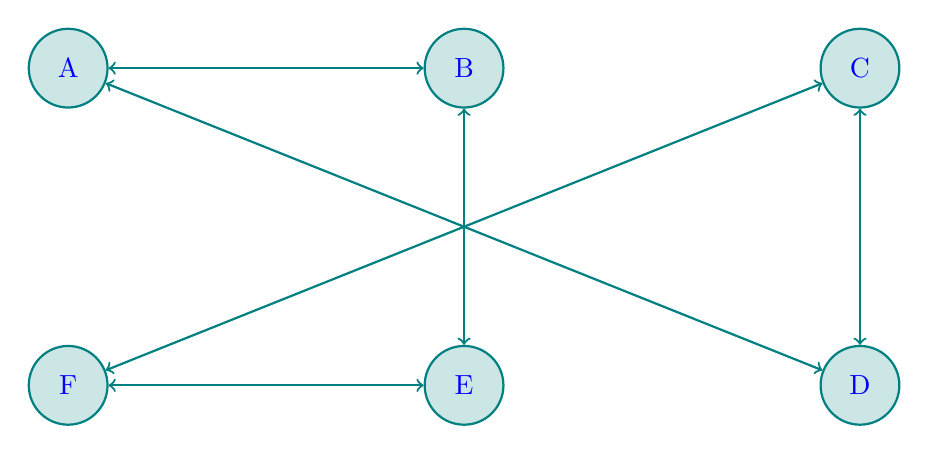
\begin{tikzpicture}[
        node distance=3cm and 4cm,
        router/.style={circle, draw, teal, text=blue, minimum width=1 cm, thick, fill=teal!20},
        link/.style={draw, teal, minimum width=1 cm, thick, <->}]
    \node[router] (A) {A};
    \node[router] (B) [right=of A] {B};
    \node[router] (C) [right=of B] {C};
    \node[router] (D) [below=of C] {D};
    \node[router] (E) [below=of B] {E};
    \node[router] (F) [below=of A] {F};
    \path[link] (A) edge node {} (B);
    \path[link] (A) edge node {} (D);
    \path[link] (B) edge node {} (E);
    \path[link] (C) edge node {} (D);
    \path[link] (C) edge node {} (F);
    \path[link] (E) edge node {} (F);
\end{tikzpicture}
\end{center}

\subsection{}
$D \rightarrow C \rightarrow F$

\subsection{}
$A \rightarrow B \rightarrow E \rightarrow F$

\section{}
Actually, there where two problems with the 2021 Facebook(aka Meta) outage. First, the backbone network of the company was disconnected from the internet because of a command mistake by an employee. Second, becuase of the later issue, the company authorative name server refused to give out the IP addresses. This is because of a implemented feature, in which authorative name servers disable those advertisements that they can not speak to. The final result was the unaccessible network of the company.

The most trivial possible attack in this situation, is the physical access to datacenters becuase of the chaos. Aside from that, some attacker could poison DNS servers and add records to his/her own servers. This way he/she can steal login credentials of the company users.

While Facebook was out of access in all of the world, the Facebook IP addresses could be resolved in the Iran. Despite there is not a official reason for this, I can say that this was because of the intensive internet filtering in the country. Since Iran has mapped Facebook IP addresses to their own filtering servers prior to the outage, the IP addresses could be resolved in Iran, but the servers were not associated with the company.

\subsubsection*{Resources}
\begin{itemize}
    \item \href{https://engineering.fb.com/2021/10/05/networking-traffic/outage-details/}{\url{https://engineering.fb.com/2021/10/05/networking-traffic/outage-details/}}
\end{itemize}

\end{document}
